% =====================================================================
%  Chapitre 3 : Chargement d'un gabarit
% =====================================================================
\chapter{Charger et organiser les gabarits}
\label{ch:gabarits}

\chapitreresume{Un site web sans HTML n'affiche rien. Dans ce chapitre, vous
découvrez le moteur de gabarits de Django, la fonction \code{render}, l'héritage
avec \code{base.html} et les inclusions. Vous transformez la page d'accueil en un
vrai gabarit, prêt à recevoir le design du chapitre suivant.}

\begin{objectifs}
\begin{itemize}
  \item Configurer le moteur de gabarits dans \code{settings.py}.
  \item Afficher un gabarit avec \code{render} et un dictionnaire de contexte.
  \item Créer un gabarit de base et des gabarits enfants avec \code{extends}.
  \item Découper l'interface en partials avec \code{include}.
  \item Construire des URL avec la balise \code{\% url \%}.
  \item Parcourir une liste avec \code{for} et afficher des conditions avec
        \code{if}.
\end{itemize}
\end{objectifs}

\section{Pourquoi des gabarits ?}

Dans le chapitre précédent, la vue renvoyait du HTML sous forme de chaîne Python.
Cette approche montre bien le mécanisme, mais elle ne tient pas longtemps :
\begin{itemize}
  \item le HTML se mélange au code Python ;
  \item les guillemets et les accents deviennent difficiles à gérer ;
  \item on ne peut pas réutiliser l'en-tête et le pied de page ;
  \item un designer ne peut pas travailler sans toucher au Python.
\end{itemize}

Un \textbf{gabarit} est un fichier HTML contenant des balises Django. La vue
prépare les données, le gabarit les affiche. C'est le principe de séparation des
responsabilités : le \og quoi \fg{} reste dans la vue, le \og comment \fg{} va dans
le gabarit.

\begin{retenir}
Une vue calcule, un gabarit affiche. Si vous êtes tenté d'écrire des requêtes à la
base ou des règles métier dans un gabarit, arrêtez-vous : cette logique doit
remonter dans la vue ou dans le modèle.
\end{retenir}

\section{Configurer le moteur de gabarits}

Django cherche les gabarits dans deux endroits :
\begin{enumerate}
  \item les dossiers listés dans \code{DIRS}, au niveau du projet ;
  \item les dossiers \code{templates/} des applications installées, si
        \code{APP\_DIRS} vaut \code{True}.
\end{enumerate}

Nous allons utiliser un dossier \code{templates/} à la racine du projet. Cela
facilite la vue d'ensemble et permet de partager \code{base.html} entre plusieurs
applications.

\begin{codebox}[python]{gesibiblio/settings.py, extrait}
TEMPLATES = [
    {
        "BACKEND": "django.template.backends.django.DjangoTemplates",
        "DIRS": [BASE_DIR / "templates"],
        "APP_DIRS": True,
        "OPTIONS": {
            "context_processors": [
                "django.template.context_processors.debug",
                "django.template.context_processors.request",
                "django.contrib.auth.context_processors.auth",
                "django.contrib.messages.context_processors.messages",
            ],
        },
    },
]
\end{codebox}

\begin{description}[leftmargin=3.6cm,style=nextline]
  \item[\code{DIRS}] Liste des dossiers supplémentaires où chercher les gabarits.
  \item[\code{APP\_DIRS}] Si \code{True}, Django cherche aussi dans
  \code{application/templates/}. C'est utile pour les applications réutilisables
  et pour l'administration.
  \item[\code{context\_processors}] Fonctions qui ajoutent automatiquement des
  variables à tous les gabarits. \code{request} ajoute l'objet \code{request},
  \code{auth} ajoute \code{user} et \code{perms}, \code{messages} ajoute les
  messages flash.
\end{description}

Créez le dossier \code{templates/} à la racine, puis les sous-dossiers :

\begin{codebox}[tree]{Arborescence des gabarits}
templates/
|-- base.html
|-- partials/
|   |-- navbar.html
|   `-- footer.html
`-- catalogue/
    |-- accueil.html
    `-- a_propos.html
\end{codebox}

\begin{bonne}
Placez les gabarits d'une application dans un sous-dossier portant le nom de
l'application : \code{templates/catalogue/accueil.html}. Si deux applications
créent un fichier \code{accueil.html}, Django choisit le premier trouvé. Le
sous-dossier évite ces collisions et rend les chemins explicites.
\end{bonne}

\section{Afficher un premier gabarit}

Modifiez la vue d'accueil pour utiliser \code{render} :

\begin{codebox}[python]{catalogue/views.py}
from django.shortcuts import render


def accueil(request):
    livres = [
        {"titre": "Le Petit Prince", "auteur": "Antoine de Saint-Exupéry"},
        {"titre": "Une si longue lettre", "auteur": "Mariama Bâ"},
        {"titre": "L'Étranger", "auteur": "Albert Camus"},
    ]
    return render(request, "catalogue/accueil.html", {"livres": livres})


def a_propos(request):
    return render(request, "catalogue/a_propos.html")
\end{codebox}

\begin{description}[leftmargin=2.8cm,style=nextline]
  \item[\code{render}] Raccourci qui charge un gabarit, le fusionne avec un
  contexte et renvoie une \code{HttpResponse}.
  \item[\code{"catalogue/accueil.html"}] Chemin du gabarit, relatif aux dossiers
  de gabarits.
  \item[\code{\{"livres": livres\}}] Contexte : un dictionnaire de variables
  accessibles dans le gabarit.
\end{description}

Créez \code{templates/catalogue/accueil.html} :

\begin{codebox}[html]{templates/catalogue/accueil.html}
<h1>Bienvenue dans GesiBiblio</h1>
<p>La bibliothèque numérique de la formation.</p>

<h2>Quelques livres</h2>
<ul>
  {% for livre in livres %}
    <li>{{ livre.titre }} par {{ livre.auteur }}</li>
  {% empty %}
    <li>Aucun livre pour le moment.</li>
  {% endfor %}
</ul>
\end{codebox}

Rechargez la page. Les trois livres s'affichent. Le gabarit ne contient que du
HTML et des balises ; la liste vient de la vue.

\begin{note}
\code{\{\{ ... \}\}} affiche une valeur. \code{\{\% ... \%\}} exécute une balise
(boucle, condition, URL, etc.). Les espaces à l'intérieur des accolades sont
facultatifs mais recommandés pour la lisibilité.
\end{note}

\section{Le gabarit de base et l'héritage}

Toutes les pages partagent le même en-tête, la même navigation et le même pied de
page. Recopier ce squelette dans chaque fichier serait une erreur. Django propose
l'héritage de gabarits.

\begin{figure}[htbp]
\centering
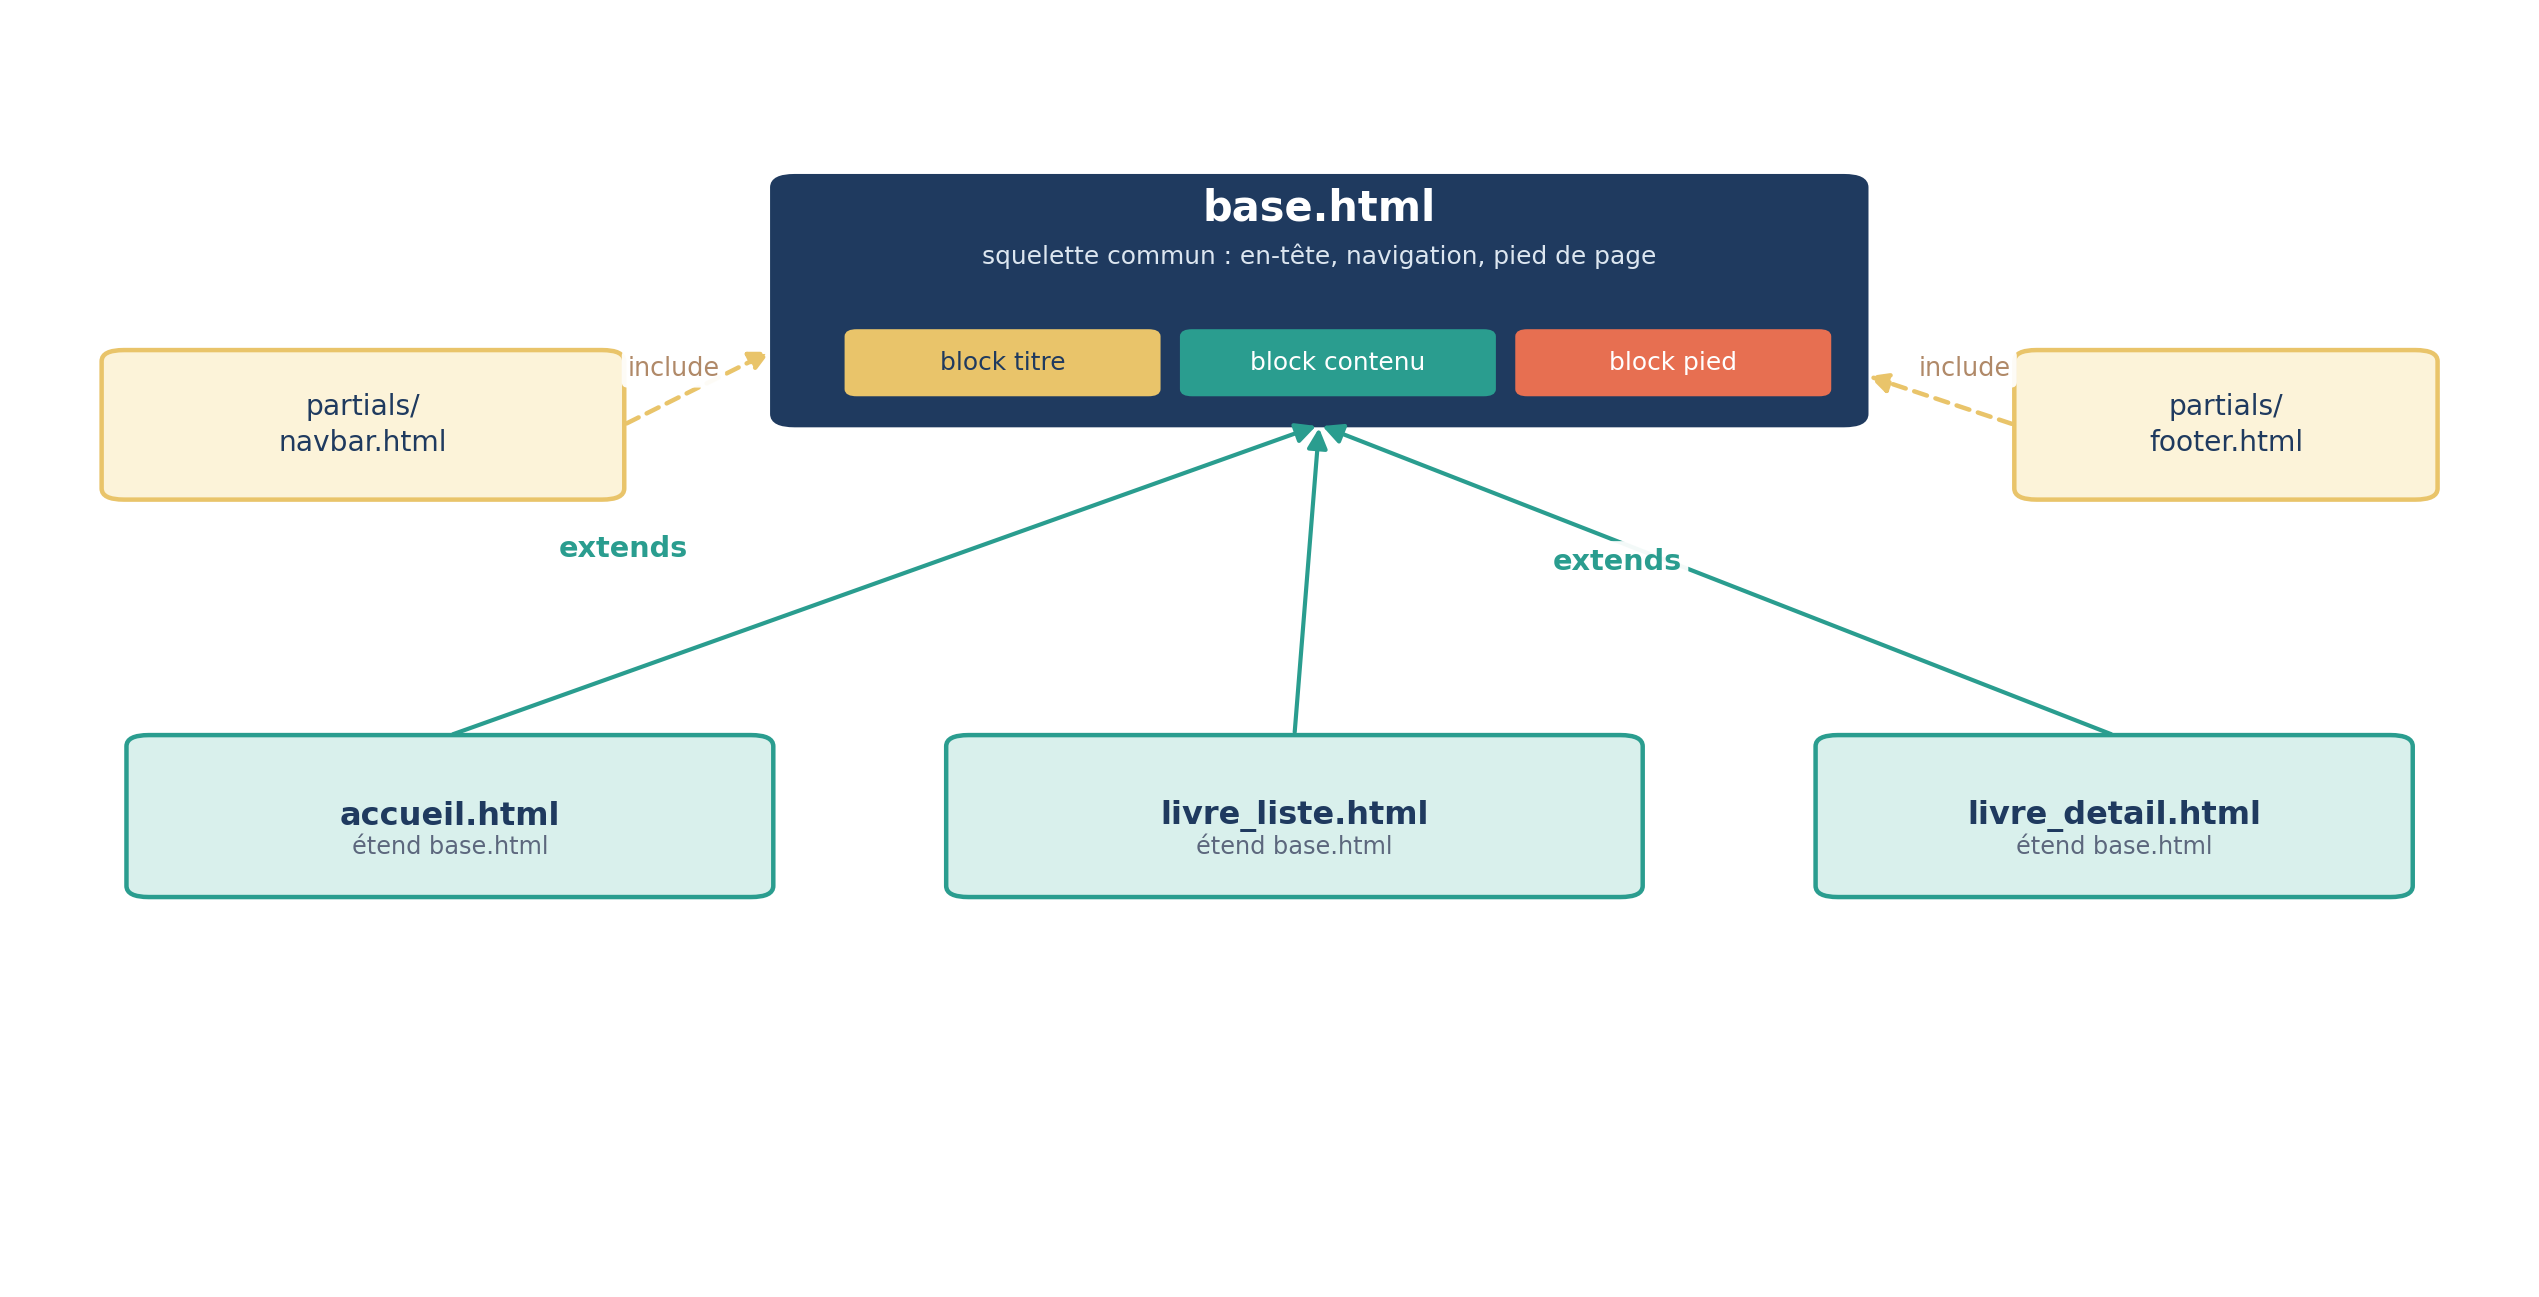
\includegraphics[width=\textwidth]{images/heritage.png}
\caption{Le gabarit \code{base.html} définit des blocs. Les gabarits enfants
remplissent ces blocs avec \code{extends}. Les partials sont inclus avec
\code{include}.}
\label{fig:heritage}
\end{figure}

\subsection{base.html}

\begin{codebox}[html]{templates/base.html}
{% load static %}
<!DOCTYPE html>
<html lang="fr">
<head>
  <meta charset="utf-8">
  <meta name="viewport" content="width=device-width, initial-scale=1">
  <title>{% block titre %}GesiBiblio{% endblock %}</title>
  <link rel="stylesheet" href="{% static 'css/style.css' %}">
</head>
<body>
  {% include "partials/navbar.html" %}

  <main class="conteneur">
    {% block contenu %}{% endblock %}
  </main>

  {% include "partials/footer.html" %}
</body>
</html>
\end{codebox}

\begin{description}[leftmargin=3.1cm,style=nextline]
  \item[\code{\{\% load static \%\}}] Charge la bibliothèque de balises
  \code{static}, nécessaire pour les fichiers CSS, JavaScript et images.
  \item[\code{\{\% block titre \%\}}] Déclare une zone que les enfants peuvent
  remplacer. Le contenu entre \code{block} et \code{endblock} est la valeur par
  défaut.
  \item[\code{\{\% block contenu \%\}}] Zone principale de la page.
  \item[\code{\{\% include \%\}}] Insère un autre gabarit à cet endroit.
\end{description}

\subsection{Les gabarits enfants}

\begin{codebox}[html]{templates/catalogue/accueil.html}
{% extends "base.html" %}

{% block titre %}Accueil | GesiBiblio{% endblock %}

{% block contenu %}
  <h1>Bienvenue dans GesiBiblio</h1>
  <p>La bibliothèque numérique de la formation.</p>

  <h2>Quelques livres</h2>
  <ul>
    {% for livre in livres %}
      <li>{{ livre.titre }} par {{ livre.auteur }}</li>
    {% empty %}
      <li>Aucun livre pour le moment.</li>
    {% endfor %}
  </ul>
{% endblock %}
\end{codebox}

\begin{codebox}[html]{templates/catalogue/a\_propos.html}
{% extends "base.html" %}

{% block titre %}À propos | GesiBiblio{% endblock %}

{% block contenu %}
  <h1>À propos</h1>
  <p>GesiBiblio est un projet de formation réalisé avec Django.</p>
  <p>Il permet de gérer un catalogue, des membres et des emprunts.</p>
{% endblock %}
\end{codebox}

\begin{attention}
\code{\{\% extends \%\}} doit être la première balise du gabarit, avant tout texte
ou espace significatif. Un fichier enfant ne peut étendre qu'un seul gabarit. Si
vous mettez du HTML avant \code{extends}, Django l'ignore ou provoque une erreur.
\end{attention}

\subsection{Le mot-clé block.super}

Si un enfant veut compléter le contenu du parent sans le remplacer, il utilise
\code{\{\{ block.super \}\}} :

\begin{codebox}[html]{Exemple de block.super}
{% block titre %}{{ block.super }} | Catalogue{% endblock %}
\end{codebox}

Le titre devient \og GesiBiblio | Catalogue \fg. C'est pratique pour ajouter un
suffixe commun à toutes les pages.

\section{Découper avec include}

Les partials sont des morceaux de gabarit réutilisables : navigation, pied de page,
carte de livre, pagination.

\begin{codebox}[html]{templates/partials/navbar.html}
<header class="entete">
  <nav class="conteneur barre">
    <a class="marque" href="{% url 'catalogue:accueil' %}">GesiBiblio</a>
    <ul class="menu">
      <li><a href="{% url 'catalogue:accueil' %}">Accueil</a></li>
      <li><a href="{% url 'catalogue:a_propos' %}">À propos</a></li>
    </ul>
  </nav>
</header>
\end{codebox}

\begin{codebox}[html]{templates/partials/footer.html}
<footer class="pied">
  <div class="conteneur">
    <p>GesiBiblio, projet de formation Django.</p>
    <p>Formation propulsée par GESITECHNOLOGIES.</p>
  </div>
</footer>
\end{codebox}

\begin{note}
Un partial hérite du contexte de la page. Si \code{navbar.html} utilise
\code{user}, la variable est disponible parce que le processeur de contexte
\code{auth} l'ajoute à tous les gabarits. Pour passer une variable spécifique,
utilisez \code{\{\% include "partial.html" with livre=livre only \%\}}. Le
\code{only} isole le partial du reste du contexte, ce qui rend ses dépendances
explicites.
\end{note}

\section{Les URL dans les gabarits}

La balise \code{url} construit une URL à partir du nom de la route :

\begin{codebox}[html]{Exemple}
<a href="{% url 'catalogue:accueil' %}">Accueil</a>
<a href="{% url 'catalogue:livre_detail' livre.slug %}">Voir le livre</a>
\end{codebox}

Le premier argument est le nom complet, préfixé par \code{app\_name}. Les arguments
suivants remplissent les paramètres de l'URL. Par exemple, si la route est
\code{path("livres/<slug:slug>/", ...)}, il faut passer le slug du livre.

\begin{bonne}
N'écrivez jamais \code{href="/livres/le-petit-prince/"} en dur. Utilisez
\code{\{\% url \%\}}. Le jour où vous changez le préfixe \code{/livres/} en
\code{/catalogue/}, toutes les pages continuent de fonctionner.
\end{bonne}

\section{Boucles et conditions}

Le langage de gabarit propose les structures de base. Voici un aperçu, détaillé au
chapitre des balises et filtres.

\begin{codebox}[html]{templates/catalogue/accueil.html, extrait}
{% if livres %}
  <ul>
    {% for livre in livres %}
      <li>
        {{ forloop.counter }}. {{ livre.titre }}
        {% if forloop.first %}(premier){% endif %}
      </li>
    {% endfor %}
  </ul>
{% else %}
  <p>Aucun livre disponible.</p>
{% endif %}
\end{codebox}

\begin{description}[leftmargin=3.3cm,style=nextline]
  \item[\code{forloop.counter}] Numéro de l'itération, à partir de 1.
  \item[\code{forloop.counter0}] Numéro de l'itération, à partir de 0.
  \item[\code{forloop.first}] Vrai pour le premier élément.
  \item[\code{forloop.last}] Vrai pour le dernier élément.
  \item[\code{\{\% empty \%\}}] Bloc exécuté si la liste est vide.
\end{description}

\section{Organiser ses gabarits}

Il existe deux emplacements possibles :
\begin{itemize}
  \item \code{templates/} à la racine du projet, pour les gabarits partagés ;
  \item \code{catalogue/templates/catalogue/} dans l'application, pour les
        gabarits propres au catalogue.
\end{itemize}

Pour ce module, nous utilisons le dossier racine \code{templates/}. C'est plus
simple à suivre pour un débutant et cela garde \code{base.html} visible. Dans un
projet réutilisable, l'emplacement dans l'application est préférable.

\begin{piege}
Un fichier \code{base.html} placé directement dans \code{templates/} est trouvé par
toutes les applications. Si vous créez plus tard une application \code{blog} qui
possède aussi un \code{base.html}, vous aurez deux fichiers concurrents. Utilisez
des noms explicites, par exemple \code{base.html} pour le site et
\code{blog/base.html} pour l'application.
\end{piege}

\section{Exercices}

\begin{exercice}[ : page À propos]
Créez le gabarit \code{templates/catalogue/a\_propos.html} et vérifiez qu'il
s'affiche à l'adresse \code{/a-propos/}. La page doit étendre \code{base.html} et
remplir le bloc \code{contenu}.
\end{exercice}

\begin{correction}
Le code est donné plus haut. Vérifiez trois points :
\begin{itemize}
  \item \code{\{\% extends "base.html" \%\}} est la première ligne ;
  \item le bloc \code{titre} est rempli ;
  \item le bloc \code{contenu} contient le HTML de la page.
\end{itemize}
Si la page est vide, vérifiez que le nom du bloc correspond exactement à celui de
\code{base.html}.
\end{correction}

\begin{exercice}[ : page Contact]
Ajoutez une page \code{/contact/} avec un gabarit qui étend \code{base.html}. La
page affiche une adresse électronique, un numéro de téléphone et les horaires.
Ajoutez le lien dans la navigation.
\end{exercice}

\begin{correction}
\begin{codebox}[python]{catalogue/views.py, extrait}
def contact(request):
    return render(request, "catalogue/contact.html")
\end{codebox}

\begin{codebox}[python]{catalogue/urls.py, extrait}
path("contact/", views.contact, name="contact"),
\end{codebox}

\begin{codebox}[html]{templates/catalogue/contact.html}
{% extends "base.html" %}

{% block titre %}Contact | GesiBiblio{% endblock %}

{% block contenu %}
  <h1>Contact</h1>
  <p>Écrivez-nous à contact@gesibiblio.example.</p>
  <p>Téléphone : 01 23 45 67 89.</p>
  <p>Ouvert du lundi au samedi, de 9 h à 18 h.</p>
{% endblock %}
\end{codebox}

Ajoutez ensuite \lstinline|<li><a href="{% url 'catalogue:contact' %}">Contact</a></li>|
dans \code{navbar.html}.
\end{correction}

\begin{exercice}[ : partial de messages]
Créez un partial \code{templates/partials/messages.html} qui affiche les messages
flash, puis incluez-le dans \code{base.html} juste après la navigation.
\end{exercice}

\begin{correction}
\begin{codebox}[html]{templates/partials/messages.html}
{% if messages %}
  <div class="conteneur messages" role="status">
    {% for message in messages %}
      <p class="message {{ message.tags }}">{{ message }}</p>
    {% endfor %}
  </div>
{% endif %}
\end{codebox}

Dans \code{base.html} :

\begin{codebox}[html]{templates/base.html, extrait}
{% include "partials/navbar.html" %}
{% include "partials/messages.html" %}
\end{codebox}

Les messages ne s'afficheront qu'après l'ajout d'un message dans une vue, par
exemple avec \code{messages.success(request, "Livre ajouté.")}.
\end{correction}

\begin{retenir}
\begin{itemize}
  \item Un gabarit est un fichier HTML enrichi de balises Django.
  \item \code{render} fusionne un gabarit et un contexte.
  \item \code{extends} et \code{block} permettent l'héritage.
  \item \code{include} réutilise des morceaux d'interface.
  \item \code{url} construit les liens à partir des noms de routes.
  \item Le gabarit affiche, il ne calcule pas.
\end{itemize}
\end{retenir}
